% Use 8.5 x 11 standard A4 paper for printing optimization in US
\documentclass[a4paper]{article}
\usepackage{float}
\marginparsep = 0pt
\marginparwidth = 0pt
\textwidth=6.5in
\oddsidemargin = 0.0in
\evensidemargin = 0.0in
\usepackage{graphicx}
\usepackage{hyperref}
\usepackage{cmbright}	% Font: Computer Modern Bright
\usepackage[T1]{fontenc}
\linespread{1.1}% spread lines out a little
\frenchspacing % remove extra space after punctuation
%\newcommand{\oscaar}{$ \texttt{OSCAAR}$ }
%\newcommand{\gui}{$ \texttt{oscaarGUI}$ }
\newcommand{\code}[1]{\texttt{#1}}
\newcommand{\init}{\code{init.par}~}
\newcommand{\oscaar}{\code{OSCAAR}~}
\newcommand{\gui}{\code{oscaarGUI}~}

\begin{document}
\title{\textbf{OSCAAR}: Open Source differential photometry Code for Amateur Astronomical Research}
\author{Brett M. Morris and the OSCAAR Team}
\maketitle
\begin{center}

\includegraphics[scale=0.3]{imgs/logoHUGEtile.png}
\end{center}
\pagebreak
\tableofcontents
\pagebreak
\section{Introduction}

\oscaar's core is a differential photometry package built for users of any experience level at observatories of any size. The process of differential photometry can be applied to many astrophysical phenomena including transiting extrasolar planets, variable stars, rotating asteroids and more. This package is prepared specially for transiting exoplanet observations, though often other photometric observations can be analyzed with \oscaar without any tweaking to the source code.

Development for \oscaar began in the summer of 2011 to take a series of images obtained at the \href{http://www.astro.umd.edu/openhouse/}{University of Maryland Observatory} in College Park, MD, USA and churn out light curves of transiting extrasolar planets. If you're looking to do something similar, you've found the right code! The core of the code is written in \href{http://www.python.org/}{Python}, but it has been designed to be operated with a graphical user interface (GUI) for users who have never seen Python before. That being said, experienced programmers will find that the guts of \oscaar provide a well-documented toolkit for even the most demanding of photometric measurements. Since the v1.0 release, \oscaar has been used by astronomers at all levels, from undergraduates to observatory-directing IAU members.

This document is intended to guide you through the observing techniques you need to make your first observations and using \oscaar to analyze them. It is currently still in the process of being written. {\bf This document is a live document, and parts may be incomplete}. We will make a stable version of the documentation for you to refer to as soon as we can!

Here we summarize the contents of this documentation. If you are new to photometry, you may consider reading Section \ref{sec:collectingData}, which will summarize observing techniques to make successful photometric measurements. In Section \ref{sec:run}, we will detail how to run \oscaar from the graphical user interface (GUI) or other ways without directly coding in Python. In Section \ref{sec:algorithmNotes} we discuss the classes and methods that are built into \oscaar that users with programming experience may find useful to design their own analysis tools. 

\subsection{System Requirements} \label{sec:systemRequirements}

There are several packages in addition to Python (v2.7) that must be installed on your machine before running \oscaar. They are all free and available for download via links below. We apologize for the number of packages that are necessary to download before using \oscaar, but we think that these packages enable for the most efficient open-source distro that we can provide.  We think you'll find that if you're going to build on the code within \oscaar, this palette of packages provides most of the tools you need for scientific computation in Python. \\ \\
\noindent
\indent \href{http://www.python.org/getit/}{\textbf{Python 2.7} (\textit{not v3.0+})}: The core language of oscaar \\
\indent \href{http://new.scipy.org/download.html}{\textbf{NumPy} and \textbf{SciPy}}: Python modules for efficient scientific computations \\
\indent \href{http://www.stsci.edu/resources/software_hardware/pyfits/}{\textbf{PyFITS 3.1.0+}}: A Python module for reading/writing FITS files \\
\indent \href{http://matplotlib.sourceforge.net/index.html}{\textbf{matplotlib}}: A Python module for publication quality, interactive plotting\\
\indent \href{http://www.wxpython.org/download.php#stable}{\textbf{wxPython 2.8+}}: A Python GUI toolkit \\
\indent \href{http://rhodesmill.org/pyephem/}{\textbf{PyEphem}}: A Python module for ephemeris calculations\\
\indent \textit{Windows only} --- \href{https://pypi.python.org/pypi/setuptools}{\textbf{setuptools}}: A Python module for installing the \oscaar package\\

\noindent Though the modules used in this package have been stable historically and probably will not go away any time soon, we want to note here that changes implemented in future versions of these packages could potentially break features in \oscaar. If you notice a broken feature, let us know by posting an issue on our Issue Tracker (see Section \ref{sec:issues}).

\subsection{Installing \oscaar}
\oscaar is currently in beta release, so there is no ``stable'' package to download just yet. Instead, each copy that you download will have the latest up-to-the-second updates. To download \oscaar via GitHub, go to \href{https://github.com/OSCAAR/OSCAAR/zipball/master}{http://github.com/OSCAAR/OSCAAR/zipball/master} to begin downloading and unarchive the ``.zip'' file. Next, open up your Command Prompt (Windows) or Terminal (Mac OS/Linux) and go to the unarchived ``OSCAAR-master'' directory (using commands like \code{cd}). Once there, type 
\begin{verbatim}
python setup.py install
\end{verbatim}
\noindent to install \oscaar in your system's Python directories. If you are working on an account without administrative privileges, you can add the \code{user} option to download \oscaar to only your user python directories:
\begin{verbatim}
python setup.py install --user
\end{verbatim}
Next, change directories to some other directory. If you were to import \oscaar from this ``OSCAAR-master'' directory, Python would use the source files that you downloaded, rather than the ones you installed. Since installation builds C libraries and downloads SAOImage DS9, it's important to run \oscaar from the installed directories, so change to some other directory before working with \oscaar.

\textit{Note for programmers:} For the reasons described above, if you want to develop new features for \oscaar, you can edit the source files that you downloaded in the  ``OSCAAR-master'' directory and run \oscaar from there, though be mindful of the extra work that the \code{setup.py} and \code{post\_setup.py} files do during the system install that will not be done in the  ``OSCAAR-master'' directory.

\section{Collecting Data} \label{sec:collectingData}

\subsection{Navigating The Sky} \label{sec:nav}

It is one hour before the photometric event that you want to observe, you have taken your flat fields, and you're ready to slew to your target. You punch in the RA and declination of the target, and your telescope lumbers over to that part of the sky, but you can't recognize the pattern of stars that come out on your first image. Is that star near the center of the field actually your target, or are you looking at the wrong part of the sky? 

While it is not necessary for running \oscaar, we highly recommend that you download the open-source planetarium software \href{http://www.stellarium.org/}{Stellarium} for navigating the sky and planning. This free, user-friendly package is supported on nearly every operating system and boasts some advanced features that will make it easy for you to find your targets. 

One feature of particular utility for the exoplanet community is that the object finding search bar that you use to find objects in Stellarium is linked to the professional astronomical database \href{http://simbad.harvard.edu/simbad/}{SIMBAD} to resolve nearly any object by any name. SIMBAD is updated relatively quickly, so when you want to go out and observe that new exoplanet but your old planetarium software doesn't know about the latest WASP or HAT target, Stellarium will resolve the name through SIMBAD and take you to the coordinates published for that object\footnote{Of course, this feature only works when your machine is connected to the internet, so if you do not have an internet connection at your observatory, you'll still need to query for your target before you get to the observatory, print out your star charts.}.

Stellarium also has great ``Flip Scene'' buttons that allow you to mirror flip your views of the sky to match the flips that your telescope optics do. That way you can match up your observed field of view with the stars in Stellarium without having to imagine complicated image transpositions in your head.

\subsection{Telescope Tracking}

Differential photometry is generally done on a series of images of the same patch of the sky over a long period of time. You'll need a telescope that is well polar-aligned so that the telescope's tracking keeps the stars in nearly the same spot on your detector throughout the duration of your observations. It is a tremendous challenge to align most small telescopes well enough to track a star perfectly over several hours, so \oscaar is built to monitor and correct for the drift in star positions on the detector over time. Just make sure your target object and a few comparison stars stay in the field throughout the whole observation\footnote{If you need to re-center your target in the middle of an observation, \oscaar will only be able to continue to track the stars without special code tweaking if you change the stars' centroid positions by a few pixels (i.e., $\sim$2 or 3 pixels) at a time in between each exposure. \textbf{The current version of \oscaar is not resilient against sudden discontinuous tracking anomalies.}}. The star tracking algorithm follows each star individually over time. If your photometric target is an asteroid, for example, that moves relative to the comparison stars over time, \oscaar will happily track the asteroid and the comparison stars independently. 

\subsection{Defocusing} \label{sec:defocusing}

In precision photometry, relying on individual pixels is dangerous. Pixel defects occur frequently that can cause a pixel to read much higher counts than they actually receive (these are called ``hot pixels'') or sometimes much lower counts (``dead pixels''). If your target object is perfectly focused on a few pixels, you may be putting all of your photometric-eggs in one basket. Thus it is often advised that you \textbf{do not focus the telescope perfectly} when doing photometric measurements. If you can, defocus the telescope significantly so that you spread out the starlight over a few of pixels, and your pixel-to-pixel variations will play a less-significant role in the introduction of unwanted systematic noise and bias. See Figure \ref{fig:defocus} for examples.

Some photometry codes prefer objects focused in Gaussian-like shapes, but \oscaar is written to accurately track stars of unconventional shapes. At the University of Maryland Observatory, we make most of our measurements on a 6in refractor. We defocus the stars until they look like small donuts (the hole is an artifact of the optical path of the refractor), and we've found that our photometry comes out best this way. \oscaar won't complain if your stars are donut-shaped, Gaussian or somewhere in between. 

\begin{figure}[H]
\begin{center}
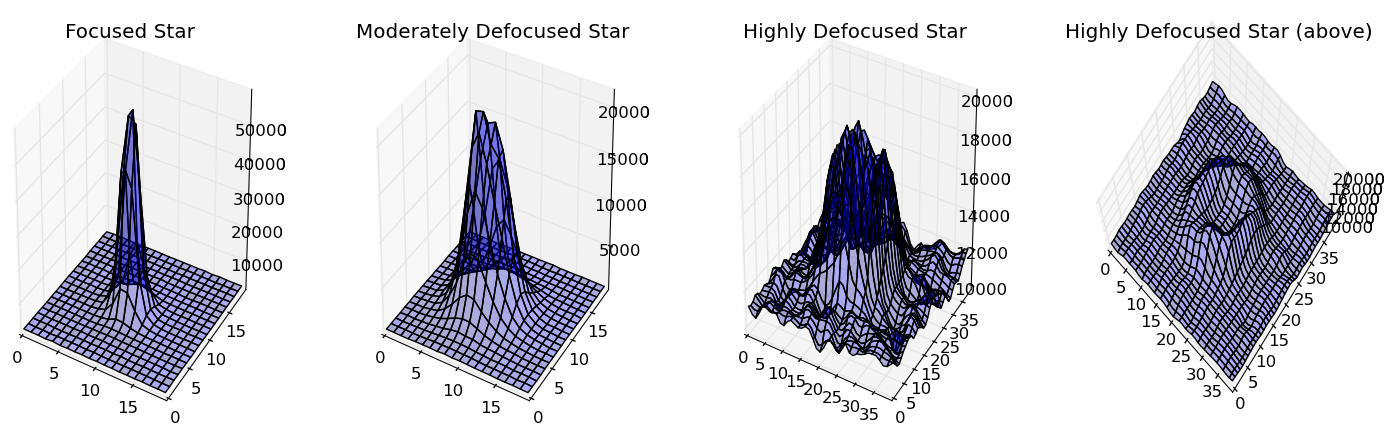
\includegraphics[scale=0.34]{imgs/focusing.png}
\caption{Images of stars with varying levels of defocusing. The $x$ and $y$ axes are the pixel indices, intensity in counts is plotted along the $z$. \oscaar can track any of these stars with precision --- even when the shape of the star is not approximately a Gaussian, like the highly defocused star on the right which is shaped like a donut.}
\label{fig:defocus}
\end{center}
\end{figure}

One must keep in mind that by spreading out the light over many pixels, the counts measured by each pixel is lower. As a result, defocusing is most helpful when observing bright objects. If the source you are observing is bright enough, you can defocus significantly without losing too much signal. However, it is important to note that the quality of your light curve will be directly related to how much more signal than noise you detected, as we will discuss in Section \ref{sec:photonNoise}. Use defocusing sparingly (or not at all) when imaging dim targets\footnote{For example, we use a sharp focus for stars dimmer than $V=10$ on our 152mm refractor at the University of Maryland Observatory.}.

\subsection{Theory: Photon Noise} \label{sec:photonNoise}

There is a fundamental physical limit to the signal-to-noise ratio that can be achieved in photometric measurements. Since photometry is the process of counting photons, there is a type of statistical uncertainty introduced into each measurement that goes by many names: \textit{photon noise, Poisson uncertainty, shot noise,} etc. This uncertainty is unavoidable in counting measurements and is easy to calculate --- the photon noise, or the uncertainty in a measurement of $N$ photons, $\sigma_N$ is

\begin{eqnarray}
\sigma_N = \sqrt{N}. \label{eqn:photonNoise}
\end{eqnarray}

\noindent You can see directly from Equation \ref{eqn:photonNoise} that the fractional uncertainty in the signal ($\sigma_N/N$) decreases with increasing $N$ as $1/\sqrt{N},$
so the more signal you have, the lower the limiting fundamental uncertainty. Of course, in practice there are many additional noise sources that will add uncertainty into your data and increase the scatter in your light curves. 
 
\subsection{Dark Fields and Flat Frames}

Collecting dark frames and flat fields is standard practice for removing systematic effects from CCD images. Flat fields correct for dust and other inconsistencies in the optical path artificially brighten or dim the objects that you image. Dark frames remove some flaws in the CCD like hot pixels and dark current variations. Some CCD imaging software like MaxIm DL have easy preset routines for taking dark frames.  We recommend taking $\ge8$ dark frames for each set of observations you take. \oscaar will take the mean of these sets and apply them appropriately to each image of your data set. 

Collecting good flat fields can sometimes be more of an art than a science, but good flats are important for good photometry. For this reason, we've incorporated two methods of ``master flat'' making routines into \oscaar, that combine raw flat fields into one master flat. The first method is called the ``Standard'' method by the \oscaar GUI, which takes a mean of all of the input flat frames. This is the fastest computational method. Standard master flats are ideal for ``dome flats'', where the flat fields are obtained by imaging a screen. Many astronomers prefer ``twilight'' or ``sky'' flats, in which the telescope takes images of the sky as the sun sets, and light from the sky acts as the uniform light source. We developed a corresponding twilight master flat setting for \oscaar, which fits a linear function to the intensity of each pixel over time, and uses the best-fit intercept as the normalizing factor for the master flat. Since loops are slow in Python, this method may take a few minutes to produce a master flat, but the payoff that you gain in photometric precision is worth the wait. At the time of writing, we're currently investigating how to implement these algorithms in \href{http://www.cython.org/}{Cython} to help us speed up these expensive computations.

%\subsection{Picking A Target}
%\subsubsection{Transit Predictions}
%So you're planning a night of transiting extrasolar planet observations, and you need to know what planets are transiting during your local night. We recommend using the \href{http://var2.astro.cz/ETD/predictions.php}{Czech Astronomical Society Exoplanet Transit Database's Transit Prediction tool}. If you enter your latitude and longitude, this web-tool will tell you which bright transiting extrasolar planets will be visible and transit on a given night from your location. This tool is invaluable for planning. It's also great because you can contribute to this database by submitting your light curves to help constrain the orbital parameters of the planets. With a telescope and \oscaar, you can contribute to real science!

%\subsubsection{Choosing The Field}
%When you chose your target for differential photometry, you need to be sure there are other stars in the imaging field. Here we'll define some terms that are important from here on:  \\ 

%\noindent \textbf{Target Star}: The target of your observations -- the host star to an exoplanet or the variable star that you're measuring for intrinsic variations in luminosity. Of course, this ``star'' could be an asteroid, if you're into that sort of thing. \\\\
%\textbf{Comparison Star}: A star other than the target star that you will use as a basis for determining the intrinsic variations in the brightness of the target star. The comparison star should be one that is not known to have intrinsic variations. \\

%There must be at least one comparison star in order to do differential photometry, and the more the better. There is no magic number of comparison stars to have, but if you have the opportunity to fit more control stars in the field by rotating your CCD or effectively ``zooming out," it will be worth your while. Based on prior experience with \oscaar, more than two good stars will suffice, but 10 can give you great results. Later, we'll discuss how to know which ones are ``good.''

%Photometry of bright stars is always preferable to dim stars, but of course there are more dim stars than bright stars in most of the images you will take. In order to avoid uncertainty introduced noise with very dim stars, pick control stars with peak intensities more than double the average background intensity in the area surrounding the star. 

%Different transiting exoplanets change the brightnesses of their host stars by different amounts. This parameter is called ``\textbf{depth}" and is often measured in units of millimagnitudes (mmag). The greater the depth of a transit, the more likely you will be capable to detect the transit. Since some of these depths are so small, you might try measuring \href{https://sites.google.com/site/aavsosppsection/}{short period pulsating (SPP) variable stars} with high amplitude luminosity oscillations (like \href{http://www.aavso.org/vsx/index.php?view=detail.top&oid=4356}{YZ Boo}) before you move on to exoplanets. Once you characterize your ability to measure the large intrinsic variations of variable stars, you will be able to characterize your ability to detect the small depth regime of transiting exoplanets. 

\subsection{Imaging Software}
A bunch of imaging packages could suite your needs for photometry with \oscaar. At the University of Maryland Observatory, we use \href{http://www.cyanogen.com/maxim_main.php}{MaxIm DL} to handle our imaging. Any imaging software that enables you to take a time-series of CCD images will do. 

Observing software like MaxIm DL allow you to choose your imaging \textbf{binning}, which enables the detector to read-out pixels in groups. For example, a $2\times2$ binning will take a square of four pixels and save them as one composite pixel. This reduces the read-out time, the size of the output files, and the run time of scripts that have to read and manipulate those images. We recommend that you use $2\times2$ binning when you can for these reasons. It is often unimportant to save images at the full-resolution of the detector, especially when you are using defocusing anyway, as described in Section \ref{sec:defocusing}. 

\section{The \oscaar GUI} \label{sec:run}

\oscaar can be run from a graphical user interface that we call the \gui. It's designed to control the running parameters that control the science algorithms so that you can tweak different features in the code by interacting with the GUI. The GUI included in \oscaar 2.0 was developed by contributor Daniel Galdi (UMD) using the \code{wxPython} package.

%\subsection{Opening the \gui}
Once \oscaar is installed, you should be able to open a Command Prompt (Windows) or Terminal (Mac OS/Linux) and type

\begin{verbatim}
python -c "from oscaar import oscaarGUI"
\end{verbatim}

\noindent to open the \gui. It will look something like Figure \ref{fig:gui}.

\begin{figure}[H]
\begin{center}
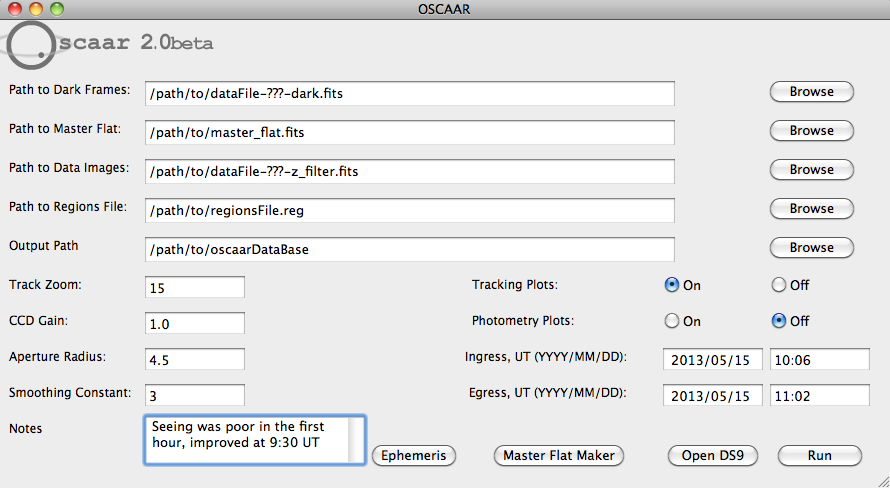
\includegraphics[scale=0.35]{imgs/GUI.png}
\caption{The \oscaar graphical user interface (GUI).}
\label{fig:gui}
\end{center}	
\end{figure}


\subsection{Transit predictions with The \oscaar Custom Ephemeris Calculator}
You've seen the weather report and you know that your observatory will have clear skies this week --- but which planets will transit this week and at what times? To answer this question, click the \code{Ephemeris} button at the bottom of the \gui.
\begin{figure}[H]
\begin{center}
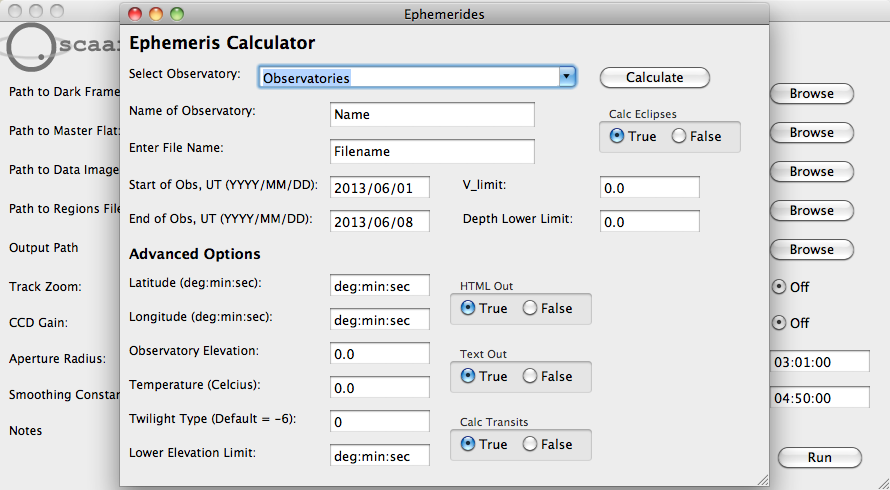
\includegraphics[scale=0.35]{imgs/ephemeris.png}
\caption{The \oscaar Custom Ephemeris Calculator.}
\label{fig:gui}
\end{center}	
\end{figure}
This new window is the \code{Ephemeris} tool, which will calculate transit time predictions for you. Select from the major observatories or friends of \oscaar listed in the \code{Select Observatory} field, or choose Enter New Observatory if yours is not listed, and enter the range of dates that you'd like to observe in the \code{Beginning of Obs} and \code{End of Obs} fields in \code{YYYY/MM/DD} format.  These dates defined in \href{http://en.wikipedia.org/wiki/Universal_time}{Universal Time (UT)}.

We've found in our experience using transit prediction services that it's easy to get drowned in too many transit event suggestions that you don't have the precision to observe. You may know, for instance, that your telescope aperture is too small or the sky brightness from light pollution at your observatory is too bright to do photometry on stars dimmer than a particular visible $V$ magnitude. We built features into this ephemeris generator so you can set the \code{$V$ upper limit} to filter out any results for transiting planets that are dimmer than a ``limiting V magnitude'' for good photometry that you've entered. At the University of Maryland Observatory, located $<15$ km from the White House and within the Washington D.C. beltway, we have plenty of light pollution. The bright sky background makes it hard to get decent photometric precision on stars with magnitudes $V>12$.

Similarly, your photometric signal-to-noise will limit the transit depths that you can observe. If a transit only causes a $10^{-4}$ fractional decrease in brightness of the star, you probably won't have the precision to be able to detect it at a small observatory. Thus you can filter out shallow (small depth) transits by setting the \code{Depth Lower Limit} field. At the University of Maryland observatory, we generally try to observe transits deeper than 0.010 magnitudes (reminder: depths are measured as positive numbers, even though they represent decreases in fluxes).

When you press \code{Calculate}, \oscaar will download a copy of the latest known transiting system parameters from \href{http://www.exoplanets.org/}{exoplanets.org}. This website created by \href{http://adsabs.harvard.edu/abs/2011PASP..123..412W}{Wright et al. (2011)} catalogs all known system parameters for each planetary system, and is updated frequently as new publications arise. \oscaar will download a copy of the entire database, and will calculate when the next transits and secondary eclipses will occur for each system using published transit times and period measurements calculate when. It also uses the right ascension and declination measurements provided by exoplanets.\@org to calculate whether or not each transit event will happen above or below the horizon, and during day or night, by performing ephemeris calculations with \code{PyEphem}. Then the transit or eclipse events that occur completely above the horizon (from ingress to egress entirely), at night, and that satisfy the $V$ limit and depth limit criteria you set are returned. 

To provide you with a consistently formatted, nicely rendered table of events, \oscaar generates the output ephemeris in HTML and opens it in your web browser. The columns of this table are sortable --- just click on the title row of each column to sort. We know that you may have this ephemeris open on your computer while you're observing at night, and we don't want you to blind yourself looking at a brightly colored ephemeris, so we included two style sheets so that you can switch between. Try changing the``Day'' to ``Night'' mode with the buttons above the ephemeris table for a dark red color palette that may disturb your night vision less than the bright ``Day'' style sheet. Outputs can also be written to CSV.

\subsubsection{Advanced Options}

The parameters in the lower half of the ephemeris calculator tool allow you to calculate the sky altitudes and directions at ingress and egress with extra-high precision, and to set the behavior of the calculator to give you more control over the results you see. The latitude and longitude of your location can be set in the format: \code{degrees:mm:ss.ss}. Your observatory elevation can be set in meters, and temperature in degrees Celsius. Then there are two parameters that will have a strong affect which transits make it through your filters. 

The \code{Twilight Type} parameter determines how many degrees below the horizon the Sun must be for \oscaar to consider the Sun to have ``set'' and for nighttime observations to begin. In practice, as you know, the sky isn't dark enough to start observations precisely at sunset, since twilight sky brightness lingers for some extra time. There are three names for different definitions of \href{http://en.wikipedia.org/wiki/Twilight#Definitions}{\textit{twilight}} --- civil, nautical and astronomical twilight, which correspond to a minimum solar elevation of $-6$, $-12$ and $-18^{\circ}$. You can chose which of these levels of solar elevation will dictate the beginning (and the end --- the same definitions work for the morning hours) of astronomical observations by tweaking this parameter. 

The \code{Lower elevation limit} parameter sets how high above the horizon the object must be before it is visible from your observatory. For photometric observations, it's a good rule of thumb to only observe objects above $30^{\circ}$ elevation, since at smaller angles the thick cross-section of air that you must look through compounds the problems of removing telluric effects.  You may, for example, have trees on the horizon in all directions at your observatory that limit your lowest-possible elevation for observing to $35^{\circ}$, or your observatory dome or roof may not accommodate observations below a similar elevation. You can account for these factors in this parameter so that you only see events that are observable with your equipment, from your observatory. The format for the \code{Lower elevation limit} parameter is  \code{degrees:mm:ss.ss}.

\subsection{Choosing Your Input Files}
The first step to running \oscaar on your data from the \gui is to select which files you want to use. \oscaar allows you to access your data files a few different ways. Our first task is to select the ``path to dark frames'' (see Figure \ref{fig:gui}). A \textit{path} is essentially a list of directions to where a file is located on your computer. On Windows you may recognize that paths to files on your hard drive are sometimes listed as ``\code{C:$\backslash$some folder$\backslash$some other folder$\backslash$...}'', and on Mac OS X they typically begin with ``\code{/Users/your user name/some folder/...}''. The easiest way to give the paths to \textit{all} of the files that you will be analyzing is to use a feature of \oscaar's path selectors that takes advantage of Python's \code{glob} module. 

The imaging software that you use may allow you to save each image from your CCD with a pre-formatted name and an iterating index for each image. For example, in our sample data set we simulate this behavior by giving all of the dark frames names with the pattern ``simulatedImg-000d.fits'', ``simulatedImg-001d.fits'', ``simulatedImg-002d.fits'', etc. You could press the \code{Browse} button in the \gui and then hold shift and click through every dark frame that you want to select, our you could use a nifty shortcut...

If you press the \code{Browse} button and select one of the dark frames, the text box to the left of the \code{Browse} will be filled with the path to that file. Let's say that this text box is filled with 
\\\\
\noindent``\code{C:$\backslash$folderA$\backslash$folderB$\backslash$simulatedImg-000d.fits}''. 
\\\\
\noindent We can use the ``?'' character to indicate a wildcard, so that any file that satisfies the rest of the pattern with any character in place of the ``?'' will be accepted. For the above example, if we enter 
\\\\
\noindent ``\code{C:$\backslash$folderA$\backslash$folderB$\backslash$simulatedImg-???d.fits}'' 
\\\\
\noindent we will get back all of the files that have that pattern with any numbers (or letters) in place of the question marks. 

Let's say all of the images in ``folderB'' are dark images, and you want to just select all of those files. You can use the ``*'' character in place of the name of the file, and all files in the directory will be selected, for example, 
\\\\
\noindent ``\code{C:$\backslash$folderA$\backslash$folderB$\backslash$*}'' 
\\\\
\noindent will grab all files in ``folderB''. But what if there was a text file or some other non-FITS file in ``folderB''? In that case, you can specify the file extension and/or last few characters so that you get the right file, like this: 
\\\\
\noindent ``\code{C:$\backslash$folderA$\backslash$folderB$\backslash$*.fits}'', 
\\\\
\noindent which will catch all FITS files in ``folderB''.

Go ahead and fill in these fields for the dark frame and data image paths. When you use any of these rules, \oscaar will figure out all files that match and use those files for you. The next time you load the \gui, the files that were grabbed will be listed in the text box, separated by commas. 

The ``Output Path'' field asks you to pick a path to the file that \oscaar will produce with the results of all of its algorithms. Pick a place where you can put this output data file.

\subsection{Locating Your Stars with DS9} \label{sec:locatingStars}

The next task you'll have to do to prepare \oscaar for analysis is to tell it what stars you care about in your images. If you have a set of images, there could be tens or hundreds of stars in each image, some of them close to the edges, some of them with binary companions; some of them ideal control stars, some of them not. In order to ensure that the stars being picked as control stars are appropriate choices, \oscaar has the user enter each of the stars into \oscaar with the help of \href{http://hea-www.harvard.edu/RD/ds9/site/Home.html}{SAOImage DS9}. 

To begin, click the \code{Open DS9} button at the bottom of the GUI (see Figure \ref{fig:gui}) to start DS9 and open the first image from the series of images you will process. Set the scale and zoom so that you can see most of the image and most of the stars in it. With the mouse set to \code{Pointer} (\code{Edit} \textgreater  \code{Pointer}), click on the target star (the exoplanet host star or variable star). A green circle will appear over the star along with a dialogue box which contains the pixel coordinates of the circle's center and radius, see Figure \ref{fig:ds9}. 
\begin{figure}[H]
\begin{center}
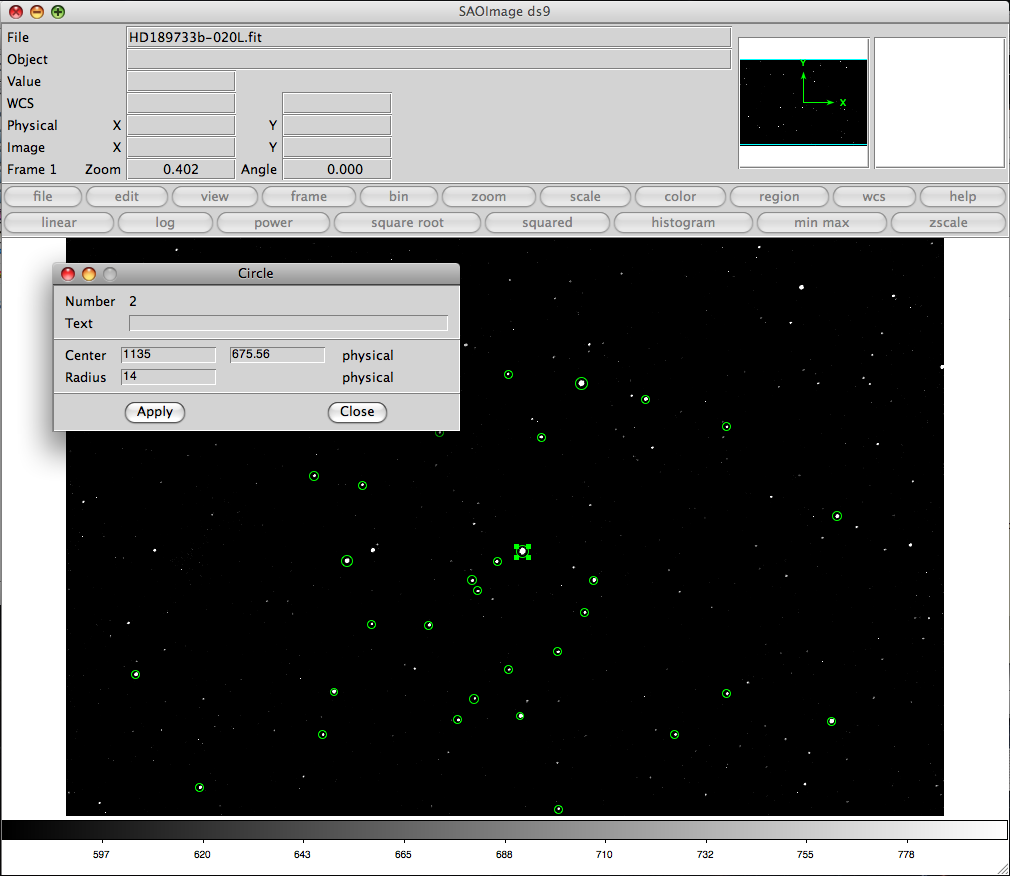
\includegraphics[scale=0.2]{imgs/ds9.png}
\caption{Using DS9 to locate the target and comparison stars.}
\label{fig:ds9}
\end{center}	
\end{figure}
The first star that you select will be treated as the target star, and any subsequent choices will be comparison stars. Repeat this process for as many comparison stars as you like (try to use as few as possible for speed). Avoid picking stars near any obvious defects on the detector, any stars less than 150 pixels from the edge of the image, or stars with a neighboring star close nearby. 

When you're done choosing control stars, go to \code{Regions} \textgreater  \code{Save Regions...} and save a regions file in a directory where you will be able to find it later. This file will contain the pixel coordinates of the stars at the beginning of the observation, which tells \oscaar which stars to track. You may want to check that the test star is in fact the first star in the regions file. Open the regions file in a text editor and check that the first line resembling ``\code{circle(100,600,10)}'' has the proper (x,y) pixel coordinates and radius (in this example, the position is (100,600) with a radius of 10). If the first circle coordinate line does not point to the target star, find the circle coordinate that does, move that line to the top of the list, and save the file. Select this regions file (with the ``.reg'' extension) from the \code{Browse} button of the \gui for the ``Path to Regions File'' field.

\subsection{Making a Master Flat}
Now that you have properly set the path to the darks and the data images, you must now make your master flat. First click the ``Master Flat Maker'' button at the bottom of the \oscaar window, and a dialog box should pop up that looks like Figure \ref{fig:flats}.
\begin{figure}[H]
\begin{center}
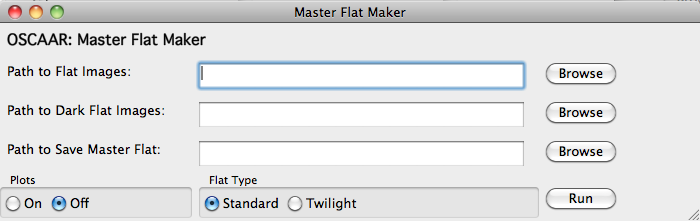
\includegraphics[scale=0.25]{imgs/flatMaker.png}
\caption{\oscaar's Master flat maker allows you to make master flats out of raw images.}
\label{fig:flats}
\end{center}	
\end{figure}

Now you must set the paths to the flat images and the dark flat images in the same way you set the image paths previously. You must also enter the path and filename for the master flat. To do this, click the \code{Browse} button and navigate to the location you would like to save the master flat. 

There are two options for how you can make your flat, either  the ``Standard'' or ``Twilight'' flat type. The standard flat maker algorithm is a simple mean combination of the flat frames that you enter into the flat maker GUI. If you took dome flats or bright sky flats, this is the right option for you. If you took flats at twilight as the sun was setting and the sky background was your ``screen'', the twilight flat algorithm will fit a linear function to the intensity of each pixel over time, and use the intercept as the normalization factor for the flat. The twilight flat algorithm is much slower than the standard method, because those linear fits are computationally expensive in an interpreted language like Python. We hope to code up alternative versions of these routines that you can experiment with on your dataset, some of which may access much faster, compiled code in C or Cython.

Now click the \code{Run} button on the master flat maker and close it when it is done. You should now choose the master flat file that you generated when selecting the ``Path to Master Flat'' in the \gui. 

\subsection{Running Parameters}
The next step in running \oscaar is to properly set all of the initial running parameters. These have default values set, but these may need to be modified for your particular data set.

\subsubsection{Smoothing Constant} \label{sec:smoothingconst}
\begin{figure}[H]
\begin{center}
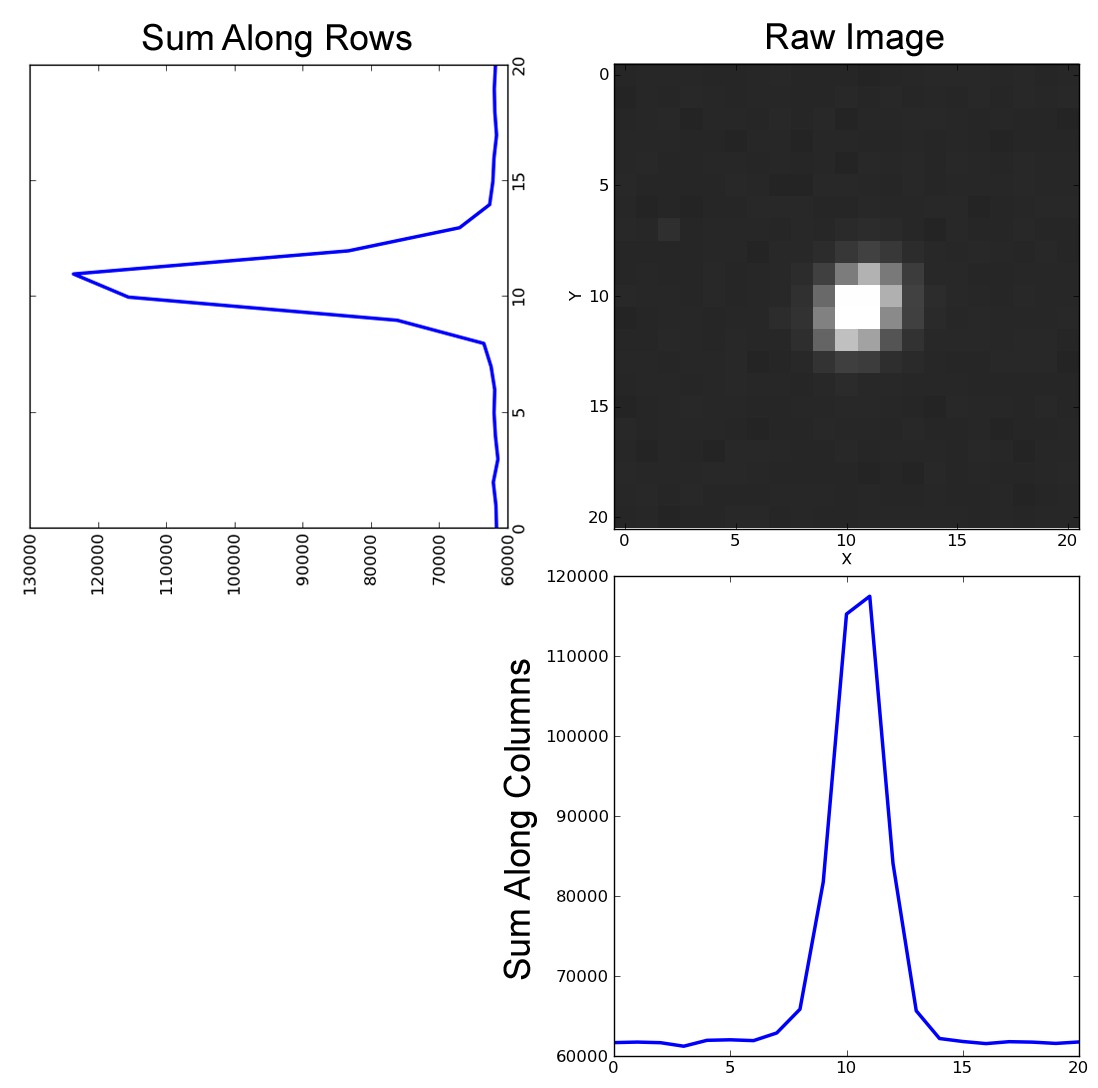
\includegraphics[scale=0.20]{imgs/sums.png}
\caption{Sums along the columns and rows around a star.}
\label{fig:sumsExample}
\end{center}	
\end{figure}
By default, oscaar v2.0 tracks stars with a fun algorithm described in Section \ref{sec:trackSmooth}. This algorithm finds the centroid of the star by looking for certain features in the first numerical derivative of the spatial intensity profile of the image of the star. These ``intensity profiles'' are the sums of pixel counts along the rows and columns near the star being tracked, see Figure \ref{fig:sumsExample} for an example. In order to find the centroids accurately using this method, it helps to smooth out the stars by blurring the image artificially, so that background noise and bad pixels are not incorrectly  interpreted as features of the stellar intensity profile. Of course, the artificial smoothing is non-destructive; the images used to measure photometry are not smoothed. 

Since it is not uncommon to defocus telescopes for photometry, you may want more or less smoothing in your images. The running parameter \code{Smoothing Constant} adjusts how much smoothing is applied in the tracking algorithm. \code{Smoothing Constant = 0} will not smooth the image at all (not recommended), and values around $\sim3$ will be significantly smeared (non-integer values are accepted). See Figure \ref{fig:smoothExample} to see what how various values of the \code{Smoothing Constant} affect a raw stellar intensity profile.
\begin{figure}[H]
\begin{center}
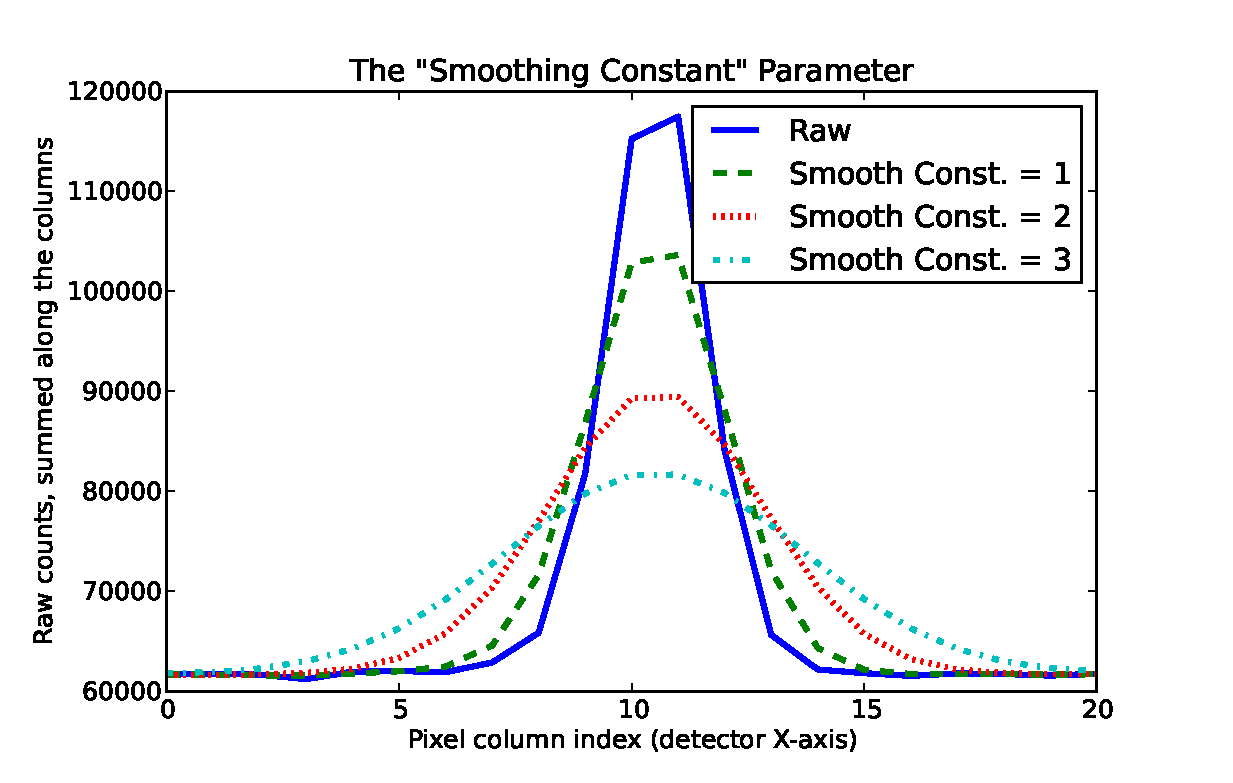
\includegraphics[scale=0.45]{imgs/smooth.eps}
\caption{A range of \code{Smoothing Constant} values from 0 to 3 are applied to the stellar intensity profile along the columns surrounding one star (see Figure \ref{fig:sumsExample} for the origin of the intensity profile).}
\label{fig:smoothExample}
\end{center}	
\end{figure}

\subsubsection{Tracking and Photometry Plots} \label{sec:trackandphotplots}
In order to visualize the effects of the running parameters that you entered on the photometric process, you can have oscaar plot visualizations of various procedures as they are executed. This will add significantly to the runtime of your analysis, as the plotting package \code{matplotlib} is not as fast as \oscaar's algorithms, however it will enable you to hone in on which running parameters you need, and allow you to troubleshoot if the results produced by oscaar are not what you expected. There are two plot settings to choose from: \code{Track plots} and \code{Photometry plots}.  \code{Track plots} will show you the centroid solutions as they are calculated in real time, along with some guide lines, see Figure \ref{fig:trackingExamples} for an example. 

\begin{figure}[H]
\begin{center}
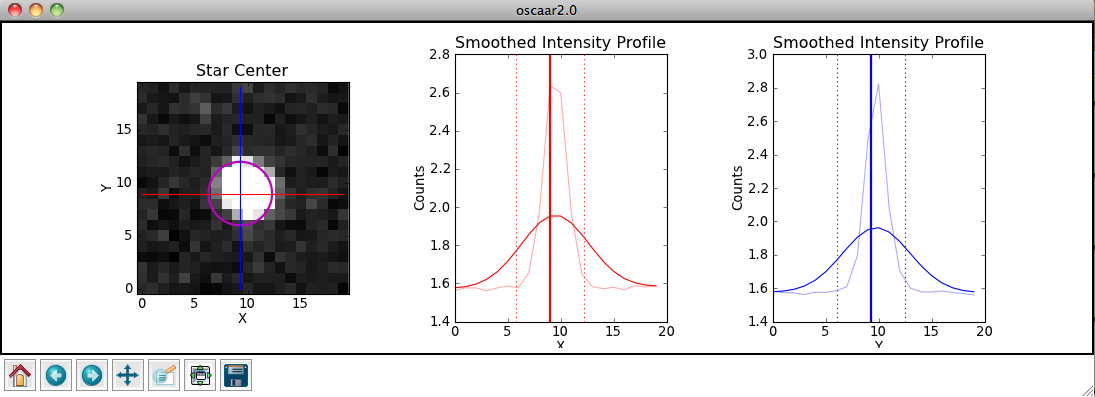
\includegraphics[scale=0.25]{imgs/trackPlots.png}
\caption{\code{Track plots} set to \code{True} and \code{Photometry plots} set to \code{False}. The leftmost image shows the star with a cross-hair indicating the centroid, also circled in magenta (the radius of this circle is not meaningful). The plots on the right indicate the sums of the intensities in pixels along the rows and columns, in the transparent curves. The solid curves represent the smoothed intensity profiles, which are used to find the centroid. The bold vertical lines mark the best-fit stellar centroid in each axis.}
\label{fig:trackingExamples}
\end{center}	
\end{figure}

\begin{figure}[H]
\begin{center}
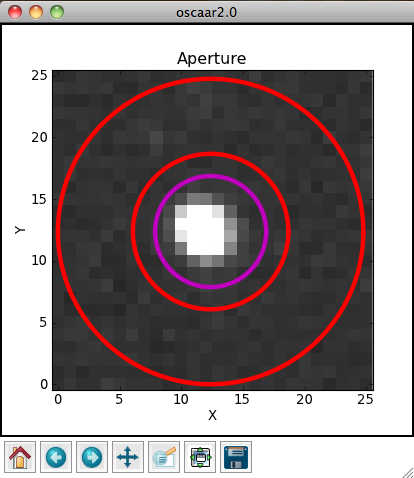
\includegraphics[scale=0.25]{imgs/aperPlots.png}
\caption{\code{Photometry plots} set \code{True} and \code{Track plots} set to \code{False}. The innermost circle (magenta) marks the \code{Aperture Radius} (see Section \ref{sec:aperRad}) measured from the stellar centroid found for this star by the tracking algorithm. All pixels that fall inside of this radius are summed to calculate the flux from this star. The next two outer concentric circles (red) circumscribe the ``sky annulus,'' within which the sky background is measured. }
\label{fig:photPlots}
\end{center}	
\end{figure}

\begin{figure}[H]
\begin{center}
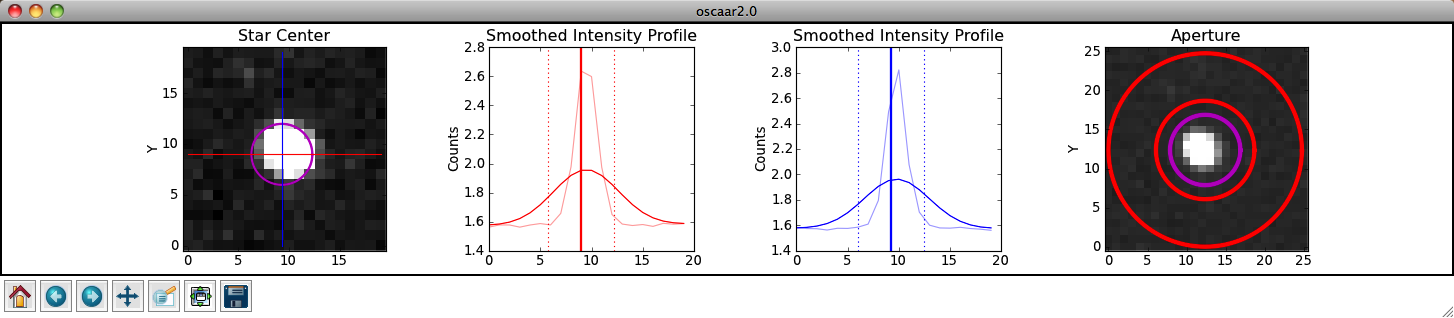
\includegraphics[scale=0.25]{imgs/trackAperPlots.png}
\caption{\code{Track plots} and \code{Photometry plots} both set \code{True}. See Figures \ref{fig:trackingExamples} and \ref{fig:photPlots} for more details on each subplot. Note: the \code{Smoothing Constant} may be too large on this image --- see for example how broad the smoothed profile is compared to the raw flux. }
\label{fig:trackAndPhotPlot}
\end{center}	
\end{figure}

\subsubsection{Track Zoom}
\oscaar tracks each star through consecutive exposures by looking for the each centroid near to the detector location that it had in the previous exposure. Since the stars will drift somewhat from frame to frame if your telescope is not perfectly aligned, we define a width around the previous centroid within which to search for the centroid in the following frame. The ideal width of this search box will depend on the plate scale of your device, how defocused the telescope is, how poor the alignment is, etc. 

See, for example, Figure \ref{fig:trackingExamples}. The \code{Track Zoom} parameter here was 20 pixels, as you can tell by the width of the image sampled along both axes. The limiting factor in how small the \code{Track Zoom} parameter should be is how far the star will move between this exposure and the next. The columns/rows where the slope of the intensity profile is at extrema (see the vertical dotted lines in Figure \ref{fig:trackingExamples}) need to fall inside of the image when cropped down to the size of \code{Track Zoom}. If the stellar centroid moved by 10 pixels in the next exposure for the star and zoom in Figure \ref{fig:trackingExamples}, \oscaar would not be able to find one of the extrema required to find the stellar centroid, and the tracking algorithm would not produce meaningful centroid estimates.

\subsubsection{CCD Gain}
The gain of a CCD is a hardware parameter that is specific to your CCD and the possible settings that you have set on it. Without getting too much into detector physics, CCDs essentially convert photons to electrons, amplify the number of electrons, and then count the amplified electrons. The number of amplified electrons counted is often more briefly referred to as the number of ``counts'', or less transparently as ``analog-to-digital units (ADU)''. If we want to be precise about how we propagate uncertainties, we need to know how many electrons were on each pixel before amplification, so the detector gain comes into our calculations. 
\begin{figure}[H]
\begin{center}
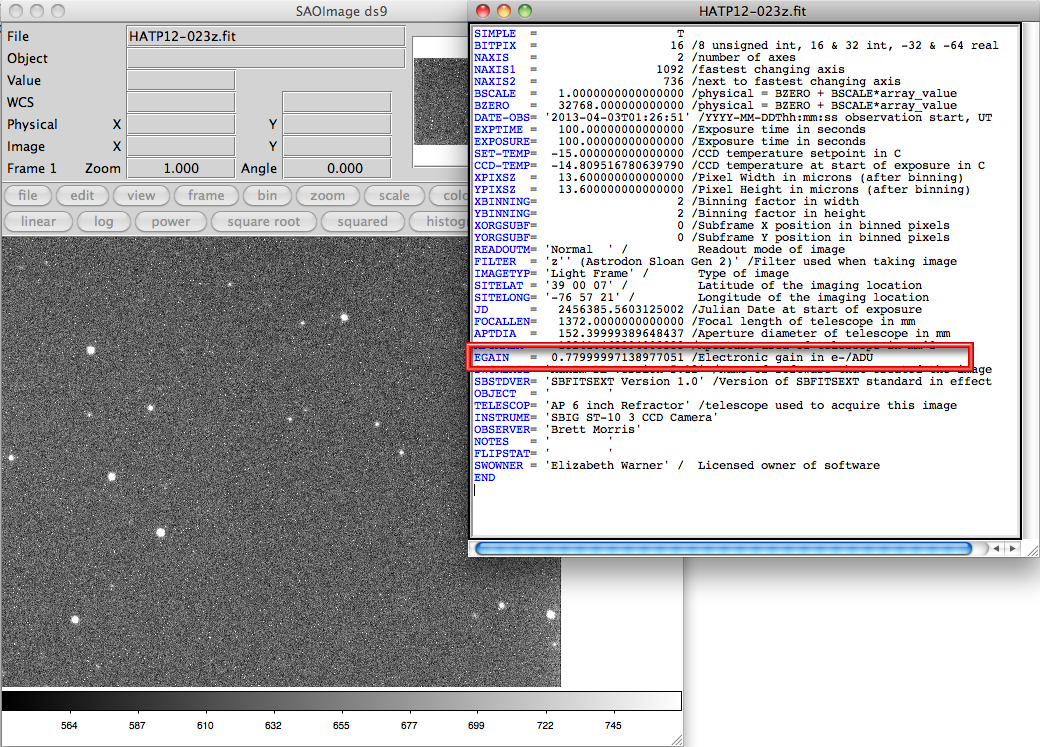
\includegraphics[scale=0.25]{imgs/ds9gain.png}
\caption{\textbf{Finding the gain}: Here's what the FITS header looks like when viewed in DS9, produced by Elizabeth Warner's 152mm refractor with an SBIG ST-10 CCD at the University of Maryland Observatory. The detector gain, labeled on this CCD as ``\code{EGAIN}'' is highlighted with a red box.}
\label{fig:ccdGain}
\end{center}	
\end{figure}
To find the gain of your detector, open one of your images in DS9. Click through the drop down menus from \code{File > Display Fits Header}. The Fits Header is a text file within each FITS file that records some notes on every exposure you take. Often there will be a line called \code{EGAIN} in there, with a comment resembling ``/ Electronic gain in e-/ADU''. This is the gain parameter to enter into oscaar. 

\subsubsection{Aperture Radius} \label{sec:aperRad}
The \code{Aperture Radius} is the radius measured outward from the stellar centroid within which we will measure the flux from the source. The \code{Aperture Radius} should fully enclose the source, and if possible, not extend any farther than necessary (though determining what is ``necessary'' may require some experimentation). 

In the duration of an observation, changes in earth's atmosphere can cause the ``width'' of a star on your detector to be larger or smaller than it was at the beginning of the night. If the star gets wider over time, the dim outer edges of the star may begin to exceed the boundaries that you set by the \code{Aperture Radius}, and some of the flux will not be counted. The differential photometry script would interpret this as the star getting dimmer, which would ruin your light curve. Therefore, when selecting the \code{Aperture Radius} parameter, we suggest that you experiment with it. Try one value with the \code{Tracking Plots} turned on (see Section \ref{sec:trackandphotplots} for details) and watch the apertures as they are applied to the images of the stars. Try a few different values (they need not be integers), and pick the smallest aperture that is sure to catch the whole star. 

\subsubsection{Notes}
This text field is meant for you to enter any notes you might want to know later. All of your running parameters will be saved in the data file so you won't need to copy them here, but if you want to label the run in any particular way, there's a great little box here specifically for that purpose.

\subsubsection{Ingress and Egress Times} \label{sec:ingEgr}
If you are observing a transiting exoplanet, \oscaar can do its most precise photometry if it knows when your target is ``in-transit'', meaning the planet is occulting the disk of star, or ``out-of-transit'', meaning the planet is not occulting the star. This is because it uses mathematical techniques that look for changes in each comparison star compared to the target star in order to determine which comparison stars are the best to use (see Section \ref{sec:calcMeanComp}). If you compared the target to comparisons while the planet was in-transit, there would be a real (and important) difference between the two that we want to measure accurately. For this reason we input the ingress and egress times and only compare the target and comparison stars during out-of-transit exposures.

Enter the times in MM/DD/YYYY;  hh:mm format, where the hours are on the 24-hour scale, in Universal Time. Seconds are insignificant.

\subsection{Results}
After you click \code{Run} and \oscaar has completed its differential photometry calculations, a light curve will pop up, like this one:
\begin{figure}[H]
\begin{center}
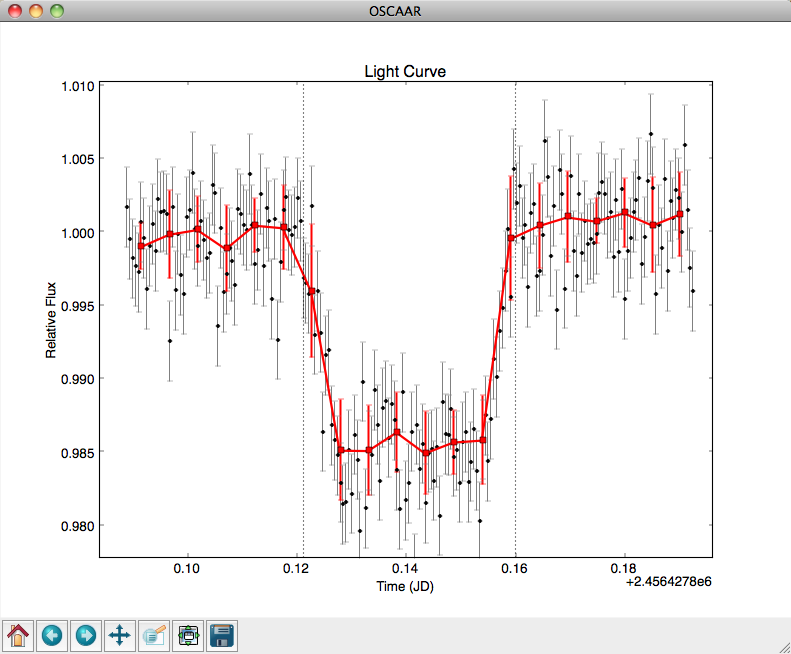
\includegraphics[scale=0.25]{imgs/lightcurve.png}
\caption{Sample light curve generated at the end of a successful \oscaar run, using sample data produced by \code{generateSampleData.py}}
\label{fig:lightcurve}
\end{center}	
\end{figure}
The black points represent the relative flux of the target star compared to the comparisons, with some uncertainty (see Figure \ref{fig:lightcurve}). The red squares bin up the black points into large bins so you can see the overall trends in noisy data. The vertical dotted lines mark the ingress and egress times that you set in Section \ref{sec:ingEgr}. 

The plot is generated with the Python package \code{matplotlib}, which supports some great interactive features. If you click the magnifying glass icon in the bottom left of the window, you can click anywhere on the plot and drag a box over a region that you'd like to zoom into. Press the home icon to return to the original view of the plot. Click the crossed-arrows icon to use the cursor to move the plot around in its box, or right click and drag to squeeze or stretch the plot. If you find that your experimentation has given you a view of the data that you'd like to hold on to, click the floppy-disk icon to save a hard copy of the plot (acceptable formats: ps, emf, gif, svg, eps, jpeg, raw, bmp, jpg, tiff, pdf, tif, png, and more). 


\subsection{Loading Previously Saved Results}
There should now be a file where you placed the ``Output Path''. If you want to look to see the raw data, or the data in various stages of processing, you can click the ``Oscaar'' drop down menu (next to \code{File} and \code{Help} at the top), and select ``Load old outputs''. The small window that pops up allows you to pick the old output file that you generated and then plot its contents in various ways. This can be useful for troubleshooting, if your light curve doesn't look the way you think it should. Light curves can be bad if the raw fluxes of one of the stars was measured improperly, for instance, so clicking the ``Plot Raw Fluxes'' button will produce a plot of the raw fluxes for each star, which may help you to debug. 


\section{Algorithm Notes} \label{sec:algorithmNotes}
\subsection{\code{oscaar.photometry.phot()}}


\subsection{\code{oscaar.astrometry.trackSmooth()}} \label{sec:trackSmooth}
The ``\textbf{point spread function}'' (PSF) for a particular observing setup is the shape of the image of a perfect point source (like a star, for example), which in practice is never a perfect ``point'' --- it will always have some radial spread. For well-focused telescopes, the PSF usually resembles an Airy function, which can be well-approximated by a Gaussian. However, as suggested in Section \ref{sec:defocusing}, you may not always want to focus the telescope perfectly. Each telescope will produce a different PSF when significantly defocused, so assuming a Gaussian PSF would prevent us from using \oscaar on defocused observations. This was a problem that we found with \oscaar v1.0, so we developed a new method with some excellent advice from Professor Drake Deming.

\code{trackSmooth()} does centroid-finding by summing up the intensity of the pixels near the star along both the rows and columns. The sums along the rows and columns will produce intensity profiles in two axes similar to Figure \ref{fig:sumsExample}. One feature of these profiles that holds for even strongly defocused PSFs is the sharp rise and decline in the intensity of the star on either side of the stellar centroid. Typically there is a well-defined absolute maximum and minimum in the first numerical derivative of the sum along the columns, as in Figure \ref{fig:sumRowsAndCols}. The trick here is to take the midpoint between those extrema as the centroid, since searching for maxima and minima are computationally cheap. 
\begin{figure}[H]
\begin{center}
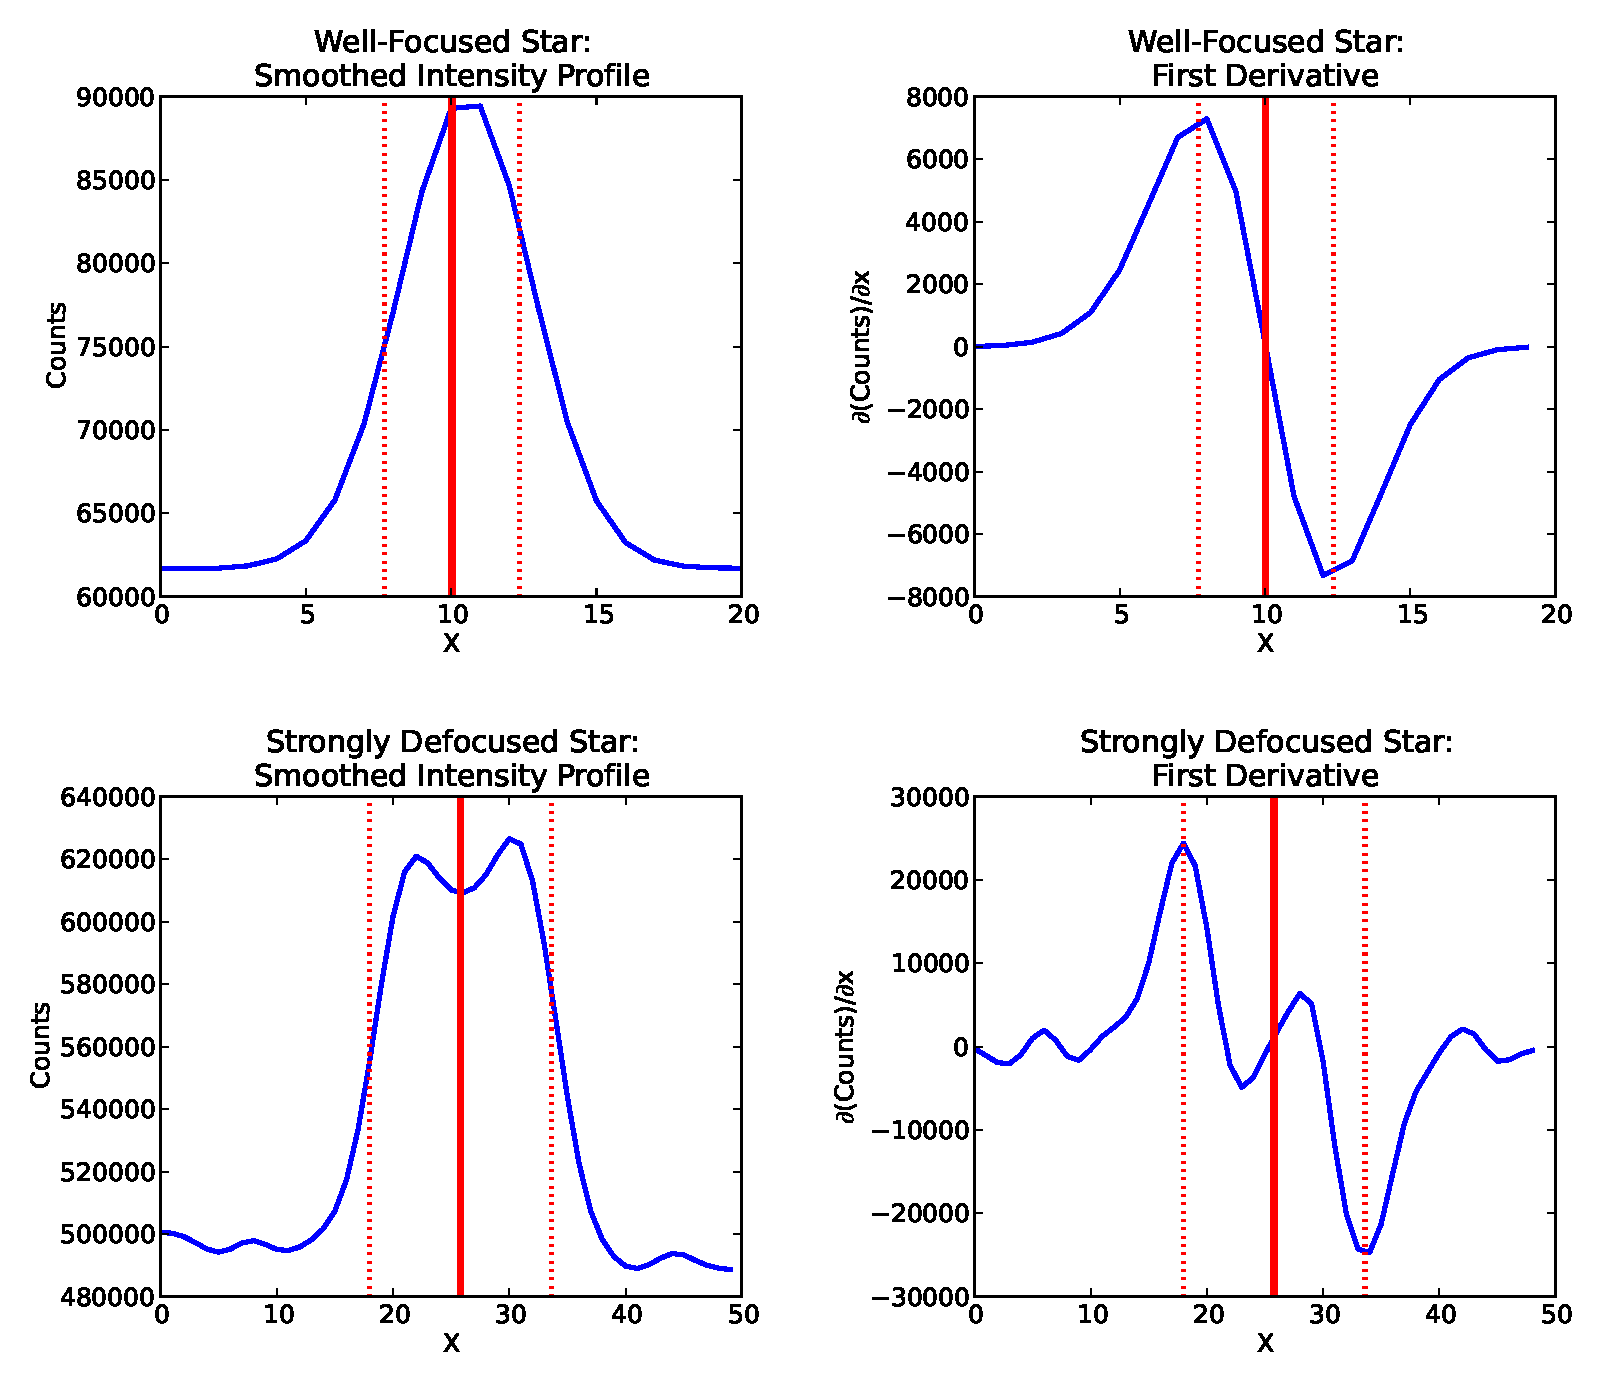
\includegraphics[scale=0.45]{imgs/trackingExample.eps}
\caption{\textbf{Stellar Centroid Tracking}: The top row of plots show the sum of intensities in each pixel along the columns a well-focus star, similar to Figure \ref{fig:sumsExample}, and the bottom row shows the same for a highly defocused star (see discussion on defocusing in Section \ref{sec:defocusing}). The plots on the left show the counts on the detector summed along the columns of pixels, and smoothed with non-zero smoothing constants. The plots on the right show the first spatial derivative of the intensity profiles, with clear extrema at the pixel locations corresponding to the points of greatest positive and negative slope in the intensity profiles. A quadratic is fit to the three points closest to each of the extrema, yielding sub-pixel precision on the coordinates of the extrema (marked above with the dotted vertical red lines). The midpoint between these best-fit extrema is taken as the stellar centroid, marked with the solid vertical red line in the plots above. This process is repeated for the other axis (sum along the rows) to get the other of the two dimensional centroid coordinates for each star.}
\label{fig:sumRowsAndCols}
\end{center}	
\end{figure}
In order to increase our centroid precision, we then use a little linear algebra to fit a quadratic to the three pixels nearest the maximum or minimum. The midpoints between the apexes of the best-fit quadratic near the maximum and minimum is taken as the centroid. This process is repeated for the sums along the rows and the columns to get the centroid in both axes. 

Observational data is never clean. There may be dead pixels or hot pixels that would appear as sharp spikes or troughs in the intensity profiles. These pixels, if unaccounted for, will appear to the tracking algorithm to be the sharp edges of a star in the image. This is why we run the image through the smoothing routine --- to smear out any sharp artifacts in the image, so that the tracking algorithm only anchors itself on the overall features of the image and not faulty individual pixels. This smoothing routine can apply varying degrees of smoothing to each image, and choosing a proper amount of smoothing is covered in Section \ref{sec:smoothingconst}. 


\subsection{The \code{dataBank} Object}
Storing and managing all of the data that comes with differential photometry scripts can be a nightmare, so we've developed the \code{dataBank} class to keep things organized. Python is an \href{https://en.wikipedia.org/wiki/Object-oriented_programming}{\textit{object oriented} language}, which means we can make \textit{objects} in it. Objects in \oscaar allow us to organize our data and the functions that we will use on those data (called \textit{methods}). 

One of the goals of \oscaar is to have lots of different methods for each analysis task so that you can try different ways of reducing your data without having to change out large chunks of code. If you used \code{trackSmooth()} to find stellar centroids (covered in Section \ref{sec:trackSmooth}), but thought a routine that fits two-dimensional gaussians to the images of the stars would work better, you could write a method for the \code{dataBank} class that would take the same input parameters as \code{trackSmooth()} and return the same outputs. Then all you would have to do is change the word ``trackSmooth'' to the name of your gaussian fitting method in the \code{differentialPhotometry.py} script to use the new algorithm. All of the other parts of the code could stay the same and it would be easy to change back to \code{trackSmooth()} if you wanted to. 

In the next subsections, we'll discuss some of the methods in the \code{dataBank} class. Since all of the photometry data is stored in this class, most of the differential photometry algorithms that manipulate the raw fluxes to calculate a light curve are written in this class as well. Therefore this section can also be though of as a play-by-play description of the standard \oscaar differential photometry routine.


\subsubsection{\code{dataBank.scaleFluxes()}}

Each star that you observe will have a different apparent magnitude, and the dimmer the star is the more significantly the flux measurements will be affected by sources of noise. If we're going to compare the flux variations of each comparison star to the target star, which all are affected by noise to different degrees, we need to make sure that we're accounting for the lower signal-to-noise ratio for the dim stars and higher signal-to-noise ratio for the bright ones. 

To accomplish this, we do a linear regression to find a multiplicative coefficient to apply to each comparison star. Multiplying this coefficient to the raw fluxes of the comparison stars ``scales their fluxes'' to the amplitude of the raw fluxes of the target star. It equally scales the scatter of those flux measurements, which has the effect of squeezing down the scatter on brighter stars after scaling or stretching out the scatter in the fluxes of dimmer 
stars. Figure \ref{fig:rawFluxes} shows the raw fluxes from three simulated stars, calculated by \oscaar, each with a different brightness. You can see the slight decrease in brightness of the target star, shown here in red, at ingress and egress (denoted by the vertical dotted lines). 
\begin{figure}[H]
\begin{center}
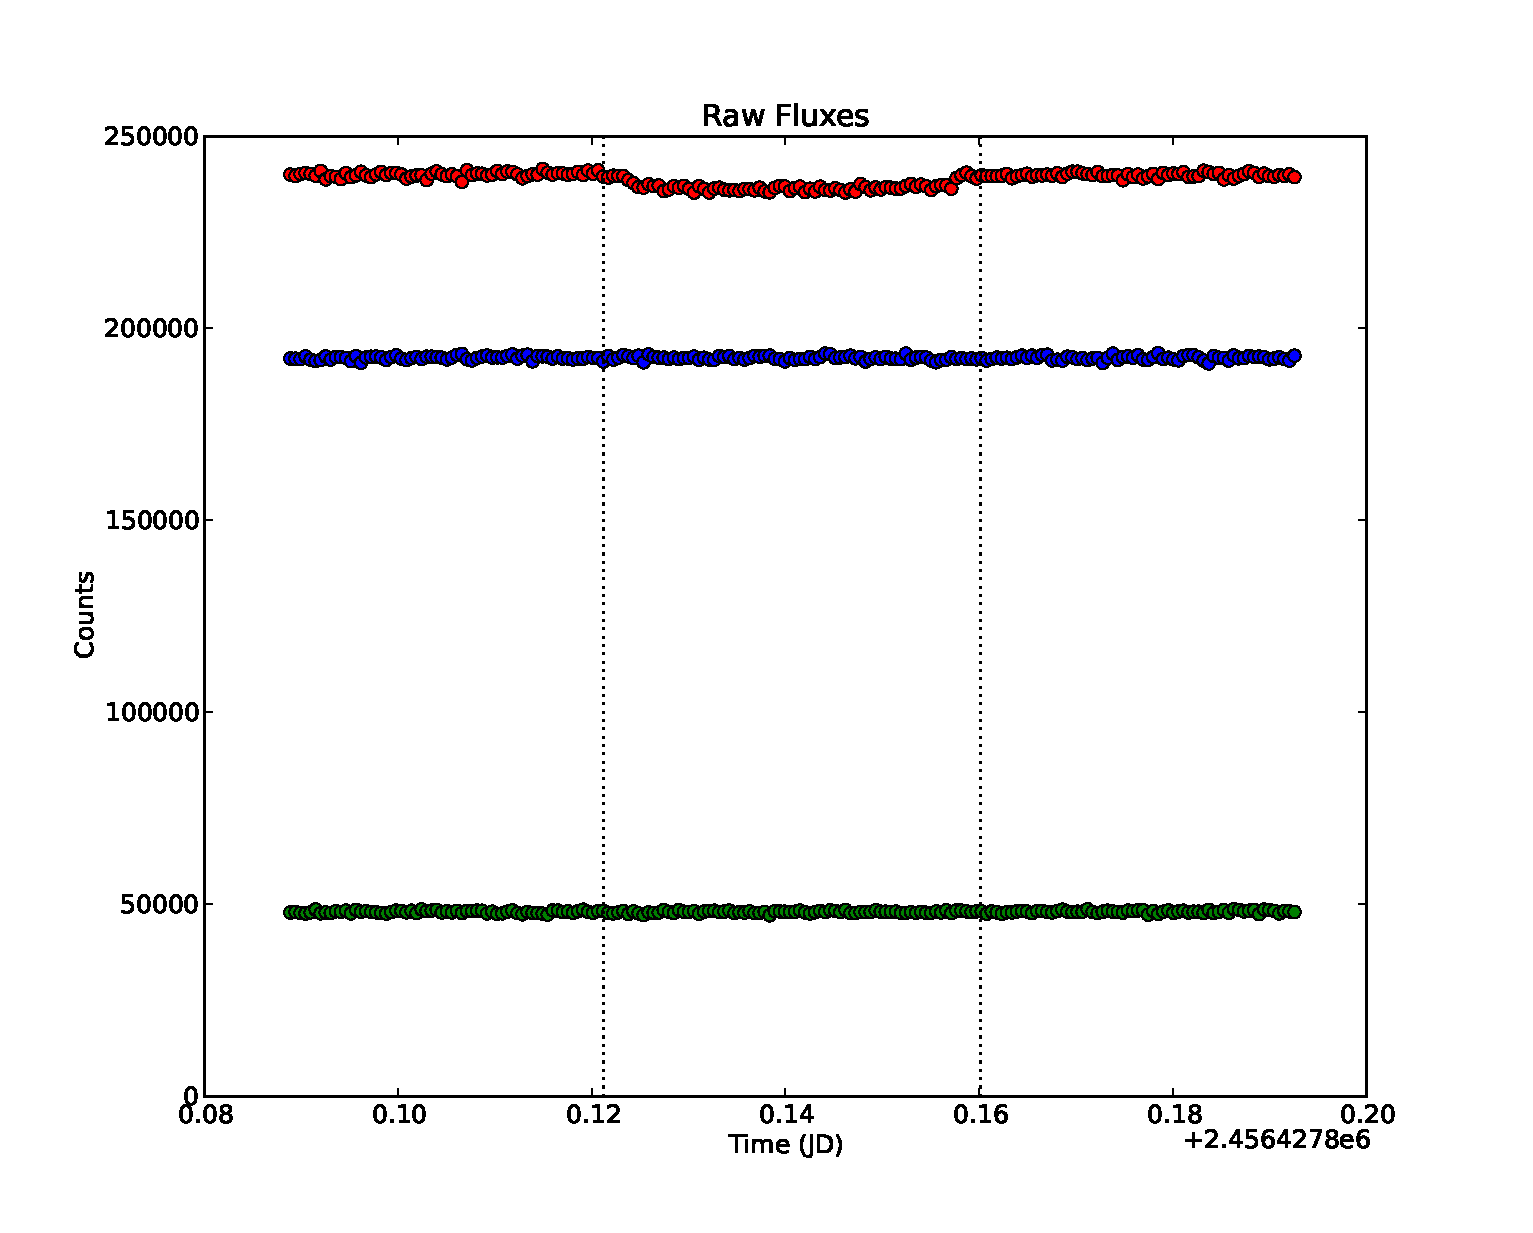
\includegraphics[scale=0.30]{imgs/rawFluxes.eps}
\caption{Raw fluxes from three simulated stars, calculated by \oscaar, each with a different brightness. You can see the slight decrease in flux of the target star, shown here in red points, at ingress and egress (denoted by the vertical dotted lines).}
\label{fig:rawFluxes}
\end{center}	
\end{figure}

\noindent When the fluxes of these comparison stars in Figure \ref{fig:rawFluxes} are run through the \code{dataBank.scaleFluxes()} routine, their fluxes get stretched to the amplitude of the target star fluxes, shown in Figure \ref{fig:scaledFluxes}. You can see that the scatter in the green comparison star's fluxes are stretched significantly larger, conserving the relative signal-to-noise ratios of each star. Now we could do a $\chi^2$ or similar analysis to compare how closely the variations in each each comparison star's fluxes match those of the target star. 

\begin{figure}[H]
\begin{center}
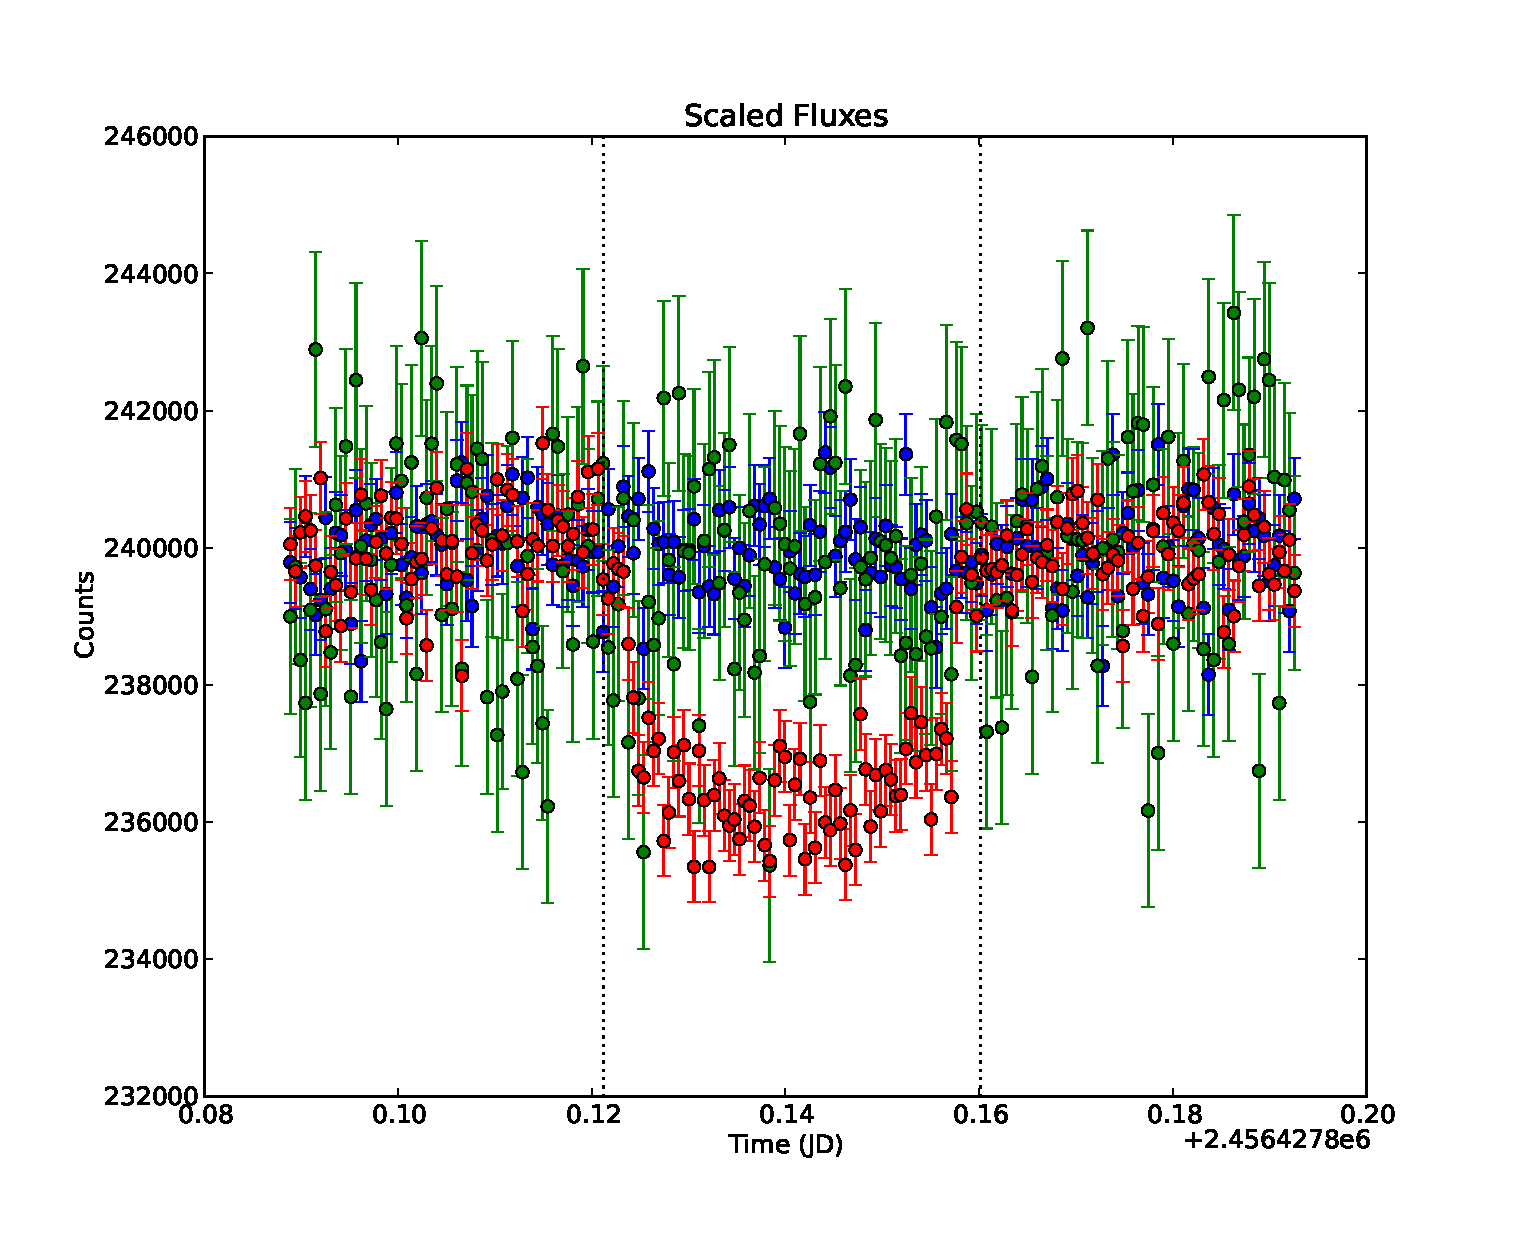
\includegraphics[scale=0.30]{imgs/scaledFluxes.eps}
\caption{Result after scaling the raw fluxes in Figure \ref{fig:rawFluxes} using the \code{dataBank.scaleFluxes()} method. Note that the fluxes of the dimmest star have the largest rms scatter, and the brightest stars have the smallest scatter after scaling.}
\label{fig:scaledFluxes}
\end{center}	
\end{figure}


\subsubsection{\code{dataBank.calcMeanComparison()}} \label{sec:calcMeanComp}

In order to make a transit light curve, we want to divide each flux measurement of the target star by the flux of a star that has no intrinsic flux variations, and ideally a star of similar spectral type to the target. How are we to know which star is the right one to use as a comparison star? To make matters worse, your detector may not be evenly responsive over the whole of the imaging surface, so stars that fall near or far away from the target star on the detector may be better to use as comparisons than others. 

We often take the mean of a bunch of comparison stars so that they can collectively make a ``composite'' comparison star, or ``mean'' comparison star, in the wording of the name of this algorithm. If one star varies a little bit or falls on a worse part of the detector, it may not introduce significant variability into the mean of the comparison stars since it gets diluted by a the non-varying fluxes of the other stars. 

Let's consider the case with two comparison stars. Ideally, we would have to perfect comparison stars imaged by a perfect detector. Their spatial positions on the CCD would not affect the measurements of their fluxes and they would have no intrinsic flux variations. In this case, the vector of mean comparison star fluxes $\mathbf{f}_{\bar{C}}$, (though unnecessary) could be produced by taking the fluxes of each comparison star $\mathbf{f}_{C,0}$ and $\mathbf{f}_{C,1}$, and taking the average: 
\begin{equation} \label{eqn:idealcomps}
\mathbf{f}_{\bar{C}} = a \cdot \mathbf{f}_{C,0}  + b \cdot \mathbf{f}_{C,1}
\end{equation}
where $a$ and $b$ here are scalar multiplier coefficients for the vectors of fluxes, with $a = b = 0.5$ in this case. We would then proceed to calculate the light curve $\mathbf{f}_{relative}$ by simple division
\begin{equation}
\mathbf{f}_{relative}  = \frac{\mathbf{f}_{T}}{\mathbf{f}_{\bar{C}}}
\end{equation}
where $\mathbf{f}_{T}$ is the vector of target fluxes. 

Now let's say that the image of the first comparison star fell on a few dead pixels on the detector, or that it has some slight intrinsic variability that does not make it a good comparison star. If we were to use Equation \ref{eqn:idealcomps} with $a = b = 0.5$ we'd be considering the first and second comparison stars with equal weight in making the mean comparison star. A more useful ``mean'' comparison star wouldn't use the mean of the two comparison stars, rather it would take some other linear combination of the fluxes with different coefficients to make the composite comparison star $\mathbf{f}_{\bar{C}}$. In this case, we would multiply the first comparison star fluxes $\mathbf{f}_{C,0}$ by a small coefficient, perhaps $a = 0.2$, and since $a + b = 1$, $b=0.8$. This will ``put a heavier weight on'' the fluxes of the second comparison star in the calculation of the mean comparison star, and should produce a better light curve. 

The \code{dataBank.calcMeanComparison()} algorithm takes the fluxes of each normalized comparison star with fluxes $\mathbf{f}_{C,i}$ and tries different weights on each star. It will minimize the difference between the out-of-transit portions of the target star fluxes and the mean comparison star fluxes by varying a set of coefficients $\mathbf{c}_i$ that get multiplied by each comparison star flux such that $\Sigma_i c_i = 1$.
\begin{eqnarray} 
\mathbf{f}_{\bar{C}} &=& c_0 \cdot \mathbf{f}_{C,0}  + c_1 \cdot \mathbf{f}_{C,1} + c_2 \cdot \mathbf{f}_{C,2} + ...\\
    &=& \Sigma_i ~ c_i \cdot \mathbf{f}_{C,i}
\end{eqnarray}
The vector of the uncertainties of the composite comparison star fluxes $\sigma \mathbf{f}_{\bar{C}}$ is then
\begin{eqnarray} 
\sigma \mathbf{f}_{\bar{C}} &=& \sqrt{ \left( c_0 \cdot \mathbf{f}_{C,0} \right)^2  + \left(  c_1 \cdot \mathbf{f}_{C,1} \right)^2+ \left( c_2 \cdot \mathbf{f}_{C,2} \right)^2+ ...} \\
     &=& \sqrt{ \Sigma_i ~ c_i^2 \cdot \mathbf{f}_{C,i}^2}
\end{eqnarray}
Of course, the out-of-transit exposures are the only ones used in this calculation because there is an important intrinsic flux variation in the target star during transit (that we're trying to see!). If we ran this regression technique to compare the target star to comparison stars on exposures taken during the transit, the algorithm would find the linear combination of target stars that best match the variability of the target star, and it would effectively seek to cancel out the transit. This is why we enter the ingress and egress times into \oscaar (see Section \ref{sec:ingEgr}), so that we can identify which exposures to use in these comparisons. 

This method also effectively cleans up after us if we choose bad comparison stars, as laid out in Section \ref{sec:locatingStars}. Let's say we chose a dim star that had a brighter nearby companion. The tracking algorithm may be able to accurately find the centroid of the dim star that we intended to use as a comparison star for a few exposures or maybe even for half of the exposures, but it may eventually ``see'' the brighter star nearby and start tracking its centroid instead. When this occurs, the flux measured for this comparison star will suddenly jump up discontinuously at the exposure when the centroid of the brighter star was found. The discontinuous flux jump in fluxes of this comparison star will be very dissimilar to continuous, telluric variations that effect the target star on a night with decent weather. The \code{dataBank.calcMeanComparison()} algorithm will find that only very small coefficients for the flux of this comparison star will produce a good composite comparison star, essentially giving this star no weight in the composite comparison star, counting it out. 

\subsubsection{\code{dataBank.computeLightCurve()}} \label{sec:computeLightCurve}
We calculate the light curve vector $\mathbf{f}_{relative}$ by simple division of the flux of the target star $\mathbf{f}_{T}$ by the flux of the composite comparison star $\mathbf{f}_{C}$, generated using \code{dataBank.calcMeanComparison()} (see Section \ref{sec:calcMeanComp}).
\begin{equation}
\mathbf{f}_{relative}  = \frac{\mathbf{f}_{T}}{\mathbf{f}_{\bar{C}}}
\end{equation}
The errors for each light curve flux are calculated by propagating of uncertainties. If $\sigma \mathbf{f}_{\bar{C}}$ is the vector of uncertainties in the composite comparison star fluxes and $\sigma \mathbf{f}_{T}$ is the vector of uncertainties in the fluxes of the target star, the uncertainties in the light curve fluxes $\sigma \mathbf{f}_{relative}$ are
\begin{equation}
\sigma \mathbf{f}_{relative}  = | \mathbf{f}_{relative} |  \sqrt{ \left(\frac{\sigma \mathbf{f}_{T}}{\mathbf{f}_{T}} \right)^2 + \left(\frac{\sigma \mathbf{f}_{\bar{C}}}{\mathbf{f}_{\bar{C}}} \right)^2 }.
\end{equation}

\section{Troubleshooting} \label{sec:issues}
If you notice a problem in \oscaar or can't get something to function properly, feel free to submit an issue on \href{https://github.com/OSCAAR/OSCAAR/issues?state=open}{our Issue Tracker on GitHub}. 

\section{Contributing to \oscaar}
This version of \oscaar was made by a very small group people, and we're proud of the work we've done. But \oscaar can still be improved and we need your help! \oscaar is used around the world by amateurs and professionals alike, and in order to keep up with the demands of providing a user-friendly differential photometry code for an international audience, we'd love to have your help if you can code in Python, or provide any feedback at all. If you'd like to help but don't know where to begin, please feel free to contact us at \href{mailto:oscaarteam@gmail.com}{oscaarteam@gmail.com}. 

\oscaar started as one of Brett Morris's independent undergraduate research projects at the University of Maryland, and since then has fueled independent research projects for several other undergraduates. If you are an undergraduate studying astronomy, physics or computer science and would like to contribute to oscaar, we encourage you to reach out to us. We'd love to work together! 

We keep the \href{https://github.com/OSCAAR/OSCAAR}{source code on GitHub}, a popular open source code repository site. There you can find the code in its most up-to-date (alpha, beta, and stable) form, the \href{https://github.com/OSCAAR/OSCAAR/issues?state=open}{Issue Tracker} where known issues are logged and new issues or comments can be posted.


\section{Acknowledgements}
\oscaar has come a long way from the first iteration that Brett Morris wrote in 2011. It could not have gotten there without the help of the following advisors and colleagues: 
Professor Drake Deming, Dr. Avi Mandell, Daniel Galdi, Sam Gross, Luuk Visser, Harley Katz, Elizabeth Warner, Professor Alberto Bolatto, Dharmatej Mikkilineni.

B.M.M. is grateful for funding that fueled a portion of this work from Dr. Avi Mandell and the Goddard Center for Astrobiology at NASA's Goddard Space Flight Center via the NASA Astrophysical Data Analysis Program. 
\end{document}